\documentclass[a4paper,fleqn,usenatbib]{mnras}
\usepackage[T1]{fontenc}
\usepackage{ae,aecompl}

\usepackage{graphicx}	
\usepackage{amsmath}	
\usepackage{amssymb}
\usepackage{tikz}
\usetikzlibrary{arrows,decorations.pathmorphing}

\title[Chirping Jets from Black Hole Binaries]{Radio Crickets:
  Chirping Jets from Black Hole Binaries Entering their Gravitational
  Wave Inspiral}

\author[Kulkarni and Loeb]{
Girish Kulkarni$^{1}$\thanks{E-mail: kulkarni@ast.cam.ac.uk}
and Abraham Loeb$^{2}$\thanks{E-mail: aloeb@cfa.harvard.edu}
\\
$^{1}$Institute of Astronomy and Kavli
  Institute of Cosmology, University of Cambridge, Madingley Road,
  Cambridge CB3 0HA, UK\\ 
$^{2}$Institute for Theory \& Computation,
  Harvard University, 60 Garden Street, Cambridge, MA 02138, USA\\ 
}

\date{Accepted ---. Received ---; in original form ---}

\pubyear{2015}

\begin{document}
\label{firstpage}
\pagerange{\pageref{firstpage}--\pageref{lastpage}}
\maketitle

\begin{abstract}
  We study a novel electromagnetic signature of supermassive black
  hole binaries whose inspiral starts being dominated by gravitational
  wave (GW) emission.  Recent simulations suggest that the binary's
  member BHs can continue to accrete gas from the circumbinary
  accretion disk in this phase of the binary's evolution, all the way
  until coalescence.  If one of the binary members produces a radio
  jet as a result of accretion, the jet precesses along a biconical
  surface due to the binary's orbital motion.  When the binary enters
  the GW phase of its evolution, the opening angle widens, the jet
  exhibits milliarcsecond scale wiggles, and the conical surface of
  jet precession is twisted due to apparant superluminal motion.  The
  rapidly increasing orbital velocity of the binary gives the jet an
  appearance of a ``chirp.''  This helical chirping morphology of the
  jet can be used to infer the binary parameters.  For binaries with
  mass $10^7$--$10^{10}$ M$_\odot$ at redshifts $z<0.5$, monitoring
  these features in current and archival data will place a lower limit
  on sources that could be detected by eLISA and Pulsar Timing Arrays.
  In the future, microarcsecond interferometry with the Square
  Kilometer Array will increase the potential usefulness of this
  technique.
\end{abstract}

\begin{keywords}
  accretion, accretion discs -- black hole physics -- quasars: supermassive black holes
\end{keywords}

\section{Introduction}
\label{sec:intro}

Binaries of supermassive black holes (BHs) arise naturally as a result
of mergers of galaxies in the context of heirarchical galaxy formation
\citep{2000MNRAS.311..576K, 2002MNRAS.336L..61H, 2008ApJ...676...33D,
  2012MNRAS.422.1306K}.  After a galaxy merger, infalling black holes
lose their angular momentum in three stages before coalescence
\citep{1980Natur.287..307B, 2005LRR.....8....8M, 2011ASL.....4..181C}.
In the first stage, the black holes sink to the center of the
gravitational potential of the merger remnant due to dynamical
friction and form a gravitationally bound binary.  The newly formed
binary then continues to lose its angular momentum and shrink by
scattering ambient gas and stars.  In the final stage of the binary's
evolution, emission of gravitational waves (GWs) becomes the
predominant mode of angular momentum loss, which results in the
coalescence of the black holes.

General relativisitic (GR) numerical simulations can predict the
binary's evolution in its final stage up to coalescence
\citep{2005PhRvL..95l1101P, 2006PhRvL..96k1102B, 2006PhRvL..96k1101C}.
This has stimulated interest in predicting related electromagnetic
signals of black hole coalescence.  Effects considered in the
literature include afterglows due to infall of gas on the remnant
black hole \citep{2005ApJ...622L..93M}, electromagnetic variability in
the circumbinary disk due to shocks induced by the sudden mass loss of
the binary following GW emission at coalescence
\citep{2007APS..APR.S1010B}, flares from shocked remnants of accretion
disk around the recoiled remnant black hole
\citep{2007PhRvL..99d1103L, 2008ApJ...682..758S, 2009CQGra..26i4032H},
quasi-periodic variability in gas accretion in the early stages of
black hole merger \citep{2008ApJ...672...83M, 2009CQGra..26i4032H,
  2012MNRAS.427.2680K}, evolution in the profiles of broad emission
lines shortly before merger \citep{2013MNRAS.432.1468M},
characteristic evolution in thermal emission due to circumbinary
accretion \citep{2015MNRAS.446L..36F}, brightening of the circumbinary
accretion disk due to viscous dissipation of gravitational waves
\citep{2008PhRvL.101d1101K}, and prompt tidal disruption of ambient
stars by the recoiled remnant \citep{2011MNRAS.412...75S}. 

In addition to testing GR in the strong field limit, observations of
electromagnetic counterparts will help localize sources of GWs for
future detectors such as the Evolved Laser Interferometer Space
Antenna (eLISA)\footnote{\url{https://www.elisascience.org}}, which
would be capable of observing the peak GW luminosity for BH
coalescence of $\sim 10^{57}$ erg$/$s out to cosmological distances
\citep{2003CQGra..20S..65H, 2013CQGra..30x4009S}.  Simultaneous
detection of GW and electromagnetic signals from coalescing binaries
will yield rich scientific pay-offs \citep{2003CQGra..20S..65H,
  2005ApJ...629...15H}.  For example, redshift measurement of eLISA
sources could constraint cosmological parameters.  Measurement of the
black hole masses and spins from the GW signal could constrain
accretion physics during coalescence.  But even before eLISA is
launched, a search of electromagnetic signatures may help calibrate
the expected abundance of GW sources.

\begin{figure}
  \begin{center}
    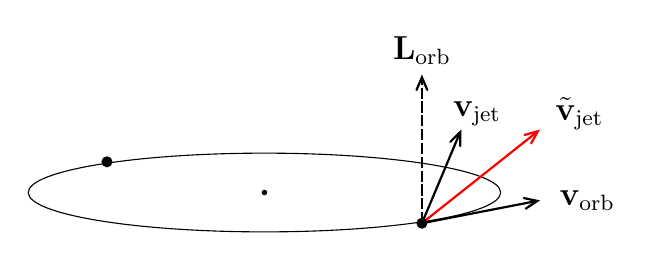
\begin{tikzpicture}
      \draw (0,0) ellipse (3 and 0.5);
      \fill[black] (0,0) circle (1pt);
      \draw [-angle 45,thick] (2,-0.39) -- (3.5,-0.1);
      \draw [-angle 45,thick,dashed,dash pattern = on 4pt off 1pt] (2,-0.39) -- (2,1.5);
      \draw [-angle 45,thick] (2,-0.39) -- (2.5,0.8);
      \draw [-angle 45,thick,red] (2,-0.39) -- (3.5,0.8);
      \fill[black] (-2,0.39) circle (2pt);
      \fill[black] (2,-0.39) circle (2pt);
      \draw (4.1,-0.1) node {\large ${\mathbf{v}}_\mathrm{orb}$};
      \draw (2.7,1.0) node {\large ${\mathbf{v}}_\mathrm{jet}$};
      \draw (4.0,1.0) node {\large $\tilde{\mathbf{v}}_\mathrm{jet}$};
      \draw (2.0,1.8) node {\large $\mathbf{L}_\mathrm{orb}$};
    \end{tikzpicture}
  \end{center}
  \caption{Jet and orbital configuration. The orbital velocity
    $\mathbf{v}_\mathrm{orb}$ causes the jet to precess as its source
    BH moves along its binary orbit. The net jet velocity is
    $\tilde{\mathbf{v}}_\mathrm{jet}={\mathbf{v}}_\mathrm{orb}+{\mathbf{v}}_\mathrm{jet}$,
    where $\mathbf{v}_\mathrm{jet}$ is its ejection velocity of the
    jet material at the source.}
  \label{fig:BH_orbit}
\end{figure}

In this Letter we study the morphology of a jet emitted by one of the
binary members during the binary's final phase of evolution before
coalescence, i.e., when the binary's dynamics is dominated by GW
emission.  We show that in this case the jet has a peculiar helical
chirping morphology that can be used to infer the binary parameters.

\section{Binary parameters}

We study a BH binary formed following a gas-rich merger of two
galaxies as a result of the processes described above.  We consider
black holes with masses $M_1$ and $M_2$ in a circular orbit of radius
$a$ around each other.  Let $M=M_1+M_2$.  For simplicity, we consider
an equal-mass binary ($M_1=M_2$) on a circular orbit. The orbital
speed of each black hole is given by \citep{2010PhRvD..81d7503L}
\begin{equation}
  v_\mathrm{orb} = \frac{1}{2}\left(\frac{GM}{a}\right)^{1/2}\!\!\!\! = 5.8\times 10^3\, \mathrm{km~s}^{-1}M_8^{1/2}a_{16}^{-1/2},
  \label{eqn:vorb}
\end{equation}
where $a_{16}\equiv (a/10^{16}$ cm$)$ and $M_8\equiv (M/10^8$
M$_\odot)$ are the binary separation and mass,
respectively.\footnote{Note that $10^{16} \mathrm{cm}\approx 3.4\times
  10^{-3} \mathrm{pc}$.  The Schwarzchild radius of a $10^8$~M$_\odot$
  black hole is $9.6\times 10^{-6}$~pc, or $\sim 3\times 10^{13}$~cm.}
The orbital period is
\begin{equation}
  P = 2\pi\left(\frac{GM}{a^3}\right)^{-1/2}\!\!\!\! = 1.72\, \mathrm{yr}\, a_{16}^{3/2} M_8^{-1/2}.
\end{equation}

In a gas-rich galaxy merger, the BH binary loses its angular momentum
by torquing the surrounding disk through spiral arms and expelling gas
out of a region twice as large as the binary orbit
\citep{2005ApJ...622L..93M, 2007PASJ...59..427H, 2008ApJ...672...83M,
  2009MNRAS.393.1423C}.  The expelled gas carries a specific angular
momentum of $\sim va$.  Further angular momentum dissipation of the
binary can happen due to its interaction with fresh gas that enters
the hollowed out region as a result of tidal torques
\citep{2008ApJ...672...83M, 2012ApJ...755...51N, 2012MNRAS.427.2680K,
  2012A&A...545A.127R}.  Therefore, the coalescence time of the binary
is inversely proportional to the rate at which fresh gas re-enters the
binary region.  But only a fraction of gas that enters the central
hollow region accretes onto the black hole and fuels quasar activity.
Therefore, we express $\dot M$ in Eddington units, $\dot{\mathcal
  M}\equiv\dot M /\dot M_E$, where $\dot M_E$ is the accretion rate
required to power the limiting Eddington luminosity with a radiative
efficiency of 10\%, $\dot M_E=2.3 M_\odot\, \mathrm{yr}^{-1}M_8$.  We
therefore have \citep{2010PhRvD..81d7503L}
\begin{equation}
  \frac{a}{\dot a} = t_\mathrm{gas}\approx\frac{J}{\dot Mva}=1.1\times 10^7\,
  \mathrm{yr}\,\dot{\mathcal M}^{-1},
\end{equation}
where $J=\mu va$ is the binary's angular momentum and $\mu=M/2$ is the
binary's reduced mass.  This time scale is greater by two orders of
magnitude than the time scale for coalescence due to angular momentum
loss by GW emission, which for circular orbits is given by
\citep{1964PhRv..136.1224P}
\begin{equation}
\frac{a}{\dot a} = t_\mathrm{GW} = \frac{5}{256}\frac{c^5a^4}{G^3M^2\mu}=2.53\times 10^5\,\mathrm{yr}\,\frac{a_{16}^4}{M_8^3}.
\end{equation}
By setting $t_\mathrm{gas}=t_\mathrm{GW}$, we can get the orbital
parameters for the binary when GWs take over.  The orbital speed at
this stage of the binary's evolution is given by
\begin{equation}
  v_\mathrm{orb} = 3.6\times 10^3\, \mathrm{km~s}^{-1}(\dot{\mathcal{M}}M_8)^{1/8},
  \label{eqn:v}
\end{equation}
The separation between the two black holes at this instant is given by
\begin{equation}
  a = 8.3\times 10^{-3}\, \mathrm{pc}\, M_8^{3/4}\dot{\mathcal{M}}^{-1/4}.
  \label{eqn:a}
\end{equation}
Note that the separation is dependent on the gas accretion rate.  

\begin{figure}
  \begin{center}
    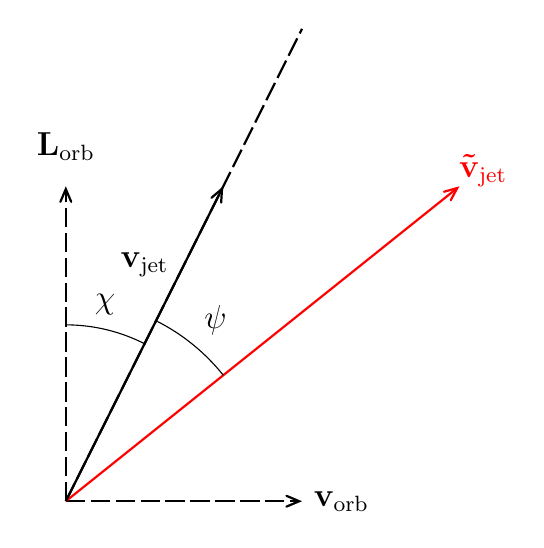
\begin{tikzpicture}
      \draw [-angle 45,dashed,thick,dash pattern = on 7pt off 2pt] (0,0) -- (3.0,0);
      \draw [-angle 45,dashed,thick,dash pattern = on 7pt off 2pt] (0,0) -- (0,4.0);
      \draw [-angle 45,thick] (0,0) -- (2.0,4.0);
      \draw [-angle 45,thick,red] (0,0) -- (5.0,4.0);
      \draw (1.0,2.0) arc (63:90:2.2);
      \draw (2.0,1.6) arc (38.6:63:2.56);
      \draw (0.5,2.5) node {\large $\chi$};
      \draw (1.90,2.3) node {\large $\psi$};
      \draw [dashed,thick,dash pattern = on 7pt off 2pt] (0,0) -- (3.0,6.0);
      \draw (0.0,4.5) node {\large $\mathbf{L}_\mathrm{orb}$};
      \draw (3.5,0.0) node {\large $\mathbf{v}_\mathrm{orb}$};
      \draw (1.0,3.0) node {\large $\mathbf{v}_\mathrm{jet}$};
      \draw (5.3,4.2) node {\large \textcolor{red}{$\mathbf{\tilde v}_\mathrm{jet}$}};
    \end{tikzpicture}
  \end{center}
  \caption{The orbital velocity $\mathbf{v}_\mathrm{orbital}$
    introduces the jet precision angle $\psi$.  Without the orbital
    motion, $\psi=0$, and the jet traces a cylindrical surface.  With
    the orbital motion, the net red velocity vector oscillates around
    the solid black vector and produces a conical surface with $\psi$
    as its half-opening angle.  Note that $v_\mathrm{orb}$ is
    exagerated here.  In practice, $v_\mathrm{orb}\ll
    v_\mathrm{jet}\sim c$.  The figure indicates that
    $\sin{\psi}\sim\tan{\psi}=v_\mathrm{orb}\cos{\chi}/v_\mathrm{jet}$.}
  \label{fig:jet}
\end{figure}

In the GW dominated phase of binary's evolution, recent simulations
show that the BHs can continue to accrete gas from the circumbinary
disk all the way until merger \citep{2015MNRAS.446L..36F}.  At this
stage, we consider a ballistic jet emanating from one of binary's
member BHs at speed $\beta=v_\mathrm{jet}/c$ at an angle $\chi$ to the
direction of the orbital angular momentum.  This geometry is depicted
in Figures~\ref{fig:BH_orbit} and \ref{fig:jet}.  As a result of the
binary orbit, the jet will wiggle on a conical surface.  (In the limit
of a small binary velocity, i.e., at large relative separations, the
jet material will move on a cylindrical surface.)  The half-opening
angle of the cone is given by \citep{1993ApJ...409..130R}
\begin{equation}
  \sin\psi = \frac{v_\mathrm{orb}\cos\chi}{v_\mathrm{jet}}.
\end{equation}

\begin{figure}
  \begin{center}
    \includegraphics*[width=\columnwidth]{evolve.pdf}
    % gw.py (case 5) 
  \end{center}
  \caption{Evolution of the binary parameters.  As the binary
    separation $a$ decreases, the orbital velocity $v_\mathrm{orb}$
    and the opening angle $\psi$ of the precessing jet, increase.
    This example describes the evolution of a binary with
    $M=10^8$~M$_\odot$ and $a_0=8.3\times 10^{-3}$~pc, but can be
    scaled to other masses and initial separations.}
  \label{fig:evolve}
\end{figure}

When the binary separation reaches the point where gravitational
wave-induced inspiral begins, the binary has a velocity given by
equation~(\ref{eqn:v}), and a separation given by
equation~(\ref{eqn:a}).  From equation (\ref{eqn:vorb}), the orbital
velocity of each BH evolves as
\begin{equation}
  \frac{\dot v_\mathrm{orb}}{v_\mathrm{orb}} = -\frac{1}{2}\frac{\dot a}{a}.
\end{equation}
which gives the evolution of the opening angle of the cone as 
\begin{equation}
 \dot\psi = -\frac{1}{2\cot\psi}\frac{\dot a}{a}.
\end{equation}
This can be solved analytically to get
\begin{equation}
  \sin\psi = \sin\psi_0\left(\frac{a_0}{a}\right)^{1/2},
\end{equation}
where $\psi_0$ and $a_0$ are the initial values. Thus, as the binary
continues to shrink the BH orbital velocity grows and the opening
angle of the conical jet increases (cone opens wider).  The rate at
which this happens reflects the binary's dynamical evolution.
Figure~\ref{fig:evolve} shows the evolution of the binary separation,
orbital velocity, and the half-opening angle for a binary in the
GW-dominated phase.

\section{Jet precession}

\begin{figure}
  \begin{center}
    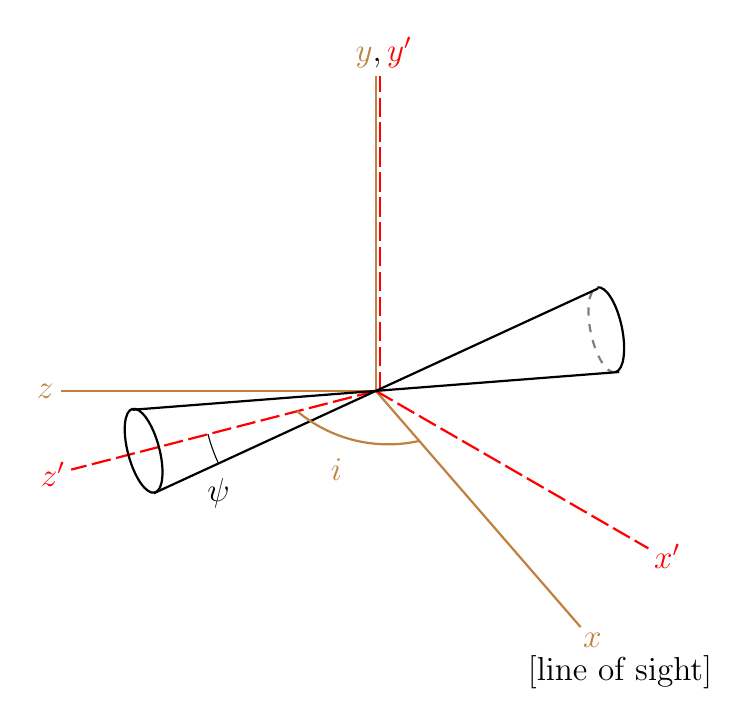
\begin{tikzpicture}
      \draw [thick,color=brown] (0,0) -- (-4.0,0);
      \draw [thick,color=brown] (0,0) -- (0,4.0);
      \draw [thick,color=brown] (0,0) -- (2.6,-3.0);
      
      \draw [dashed,thick,dash pattern = on 7pt off 2pt,color=red] (0.05,0.0) -- (0.05,4.0);
      \draw [dashed,thick,dash pattern = on 7pt off 2pt,color=red] (0,0.0) -- (3.46,-2.0);
      \draw [dashed,thick,dash pattern = on 7pt off 2pt,color=red] (0,0.0) -- (-3.87,-1.0);

      \draw [thick,rotate around={-75:(-2.95,-0.76)}] (-2.95,-0.76) ellipse (0.55 and 0.2);
      \draw [thick,rotate around={12:(3.04,0.24)}] (3.04,0.238) arc (-90:90:0.2 and 0.55);
      \draw [thick,color=gray,rotate around={12:(3.04,0.24)},dashed](3.04,0.238) arc (270:90:0.2 and 0.55);
      
      \draw [thick] (-2.82,-1.3) -- (2.82,1.3);
      \draw [thick] (-3.09,-0.24) -- (3.09,0.24);

      \draw (0.1,4.3) node {\large \textcolor{brown}{$y$},\textcolor{red}{$\,y^\prime$}};
      \draw (-4.2,0) node {\textcolor{brown}{\large $z$}};
      \draw (2.75,-3.17) node {\textcolor{brown}{\large $x$}};
      \draw (3.1,-3.57) node {\large [line of sight]};
      \draw (-4.1,-1.059) node {\large \textcolor{red}{$z^\prime$}};
      \draw (3.7,-2.1) node {\textcolor{red}{\large $x^\prime$}};

      \draw [thick,color=brown] (-1.0,-0.258) arc (230:283:1.8);
      \draw (-0.5,-1.0) node {\textcolor{brown}{\large $i$}};

      \draw (-2.0,-0.92) arc (204.75:194.48:2.2015);
      \draw (-2.0,-1.3) node {\large $\psi$};

    \end{tikzpicture}
  \end{center}
  \caption{Geometry of the jet \citep{1982ApJ...262..478G}.  The
    observer's sky is in the $yz$ plane, so that the line of sight is
    along the $x$-axis.  The jet precesses around the $z^\prime$ axis
    with half-opening angle $\psi$. The $y$ and $y^\prime$ axes
    overlap, and $z$, $x$, and $z^\prime$ axes are co-planer.  The
    angle between the $z^\prime$ axis and the line of sight is $i$.
    This geometry is valid in the limit $a\ll z^\prime\psi$.}
  \label{fig:jetgeom}
\end{figure}

\begin{figure*}
\begin{center}
  \begin{tabular}{cc}
    % jet.py (case 0) 
    \includegraphics*[scale=0.45]{{jet_i40_beta0.90_mdot1.00_full}.pdf} &
    % jet_image.py (case 1) 
    \includegraphics*[scale=0.45]{{jet_i40_beta0.90_mdot1.00_image_zoom1}.pdf}
  \end{tabular}
\end{center}
\caption{The left panel shows forward and backward jets for an
  equal-mass binary with total mass $M=10^{10}$~M$_\odot$.  We have
  assumed $i=40^\circ$, $\beta=0.9$, and angular diameter distance $d
  = 100$~Mpc.  The jets are twisted because of the apparant
  superluminal motion.  Also evident is the opening of the jet and the
  radio jet chirp.  Right panel shows normalised brightness of the
  inner 30~mas region of the forward jet.}
\label{fig:jet_mdot1.0}
\end{figure*}

We now ask if it would be possible to observe the opening of the jet
morphology.  For this purpose, it is necessary to map the above
calculations to the observer's frame \citep{1982ApJ...262..478G}.  At
a large distance compared to the binary's separation, the jet geometry
is illustrated in Figure \ref{fig:jetgeom}.  Here the source frame of
reference is shown by $x^\prime$, $y^\prime$, $z^\prime$ coordinate
systems.  The $x$, $y$, $z$ coordinate system represents the
observer's frame such that the $yz$ is the plane of the sky.  Further,
the jet is oriented such that the $y^\prime$ axis coincides with the
$y$ axis, the original direction of jet emission is at an angle $i$
relative to the line of sight ($x$-axis).  For simplicity, we also
assume that the $z^\prime$ axis is in the $xz$ plane.  Then the jet
will precess on a cone with a half-opening angle $\psi$ and an angular
velocity of precession $\Omega$.  In the source frame of reference,
the equation of the jet is then given by \citep{1981ApJ...246L.141H}
\begin{eqnarray}
  &v_x=&s_\mathrm{jet}\beta c\left[\sin\psi\sin i\cos\Omega t+\cos\psi\cos i\right],\\
  &v_y=&s_\mathrm{jet}\beta c\sin\psi\sin\Omega t,~\,\mathrm{and}\\
  &v_z=&s_\mathrm{jet}\beta c\left[\cos\psi\sin i-\sin\psi\cos i\cos\Omega t\right]. 
\end{eqnarray}
Here $s_\mathrm{jet}=\pm 1$ for forward and backward jets,
respectively.  The coordinates of a jet particle in the sky is then
given by $z=v_zt$ and $y=v_yt$.  However, because of superluminal
motion, the observer will see this on the sky as
\begin{equation}
  z=v_zt/(1-v_x/c)
\end{equation}
and
\begin{equation}
  y=v_yt/(1-v_x/c)
\end{equation}
respectively.  In angular coordinates, the motion of the jet on the
sky is given by $\phi_z=z/d$ and $\phi_y=y/d$ where $d$ is the angular
diameter distance of the binary.  Because of superluminal motion, the
forward jet is stretched while the backward jet is compressed.

Finally, we assume that the emission from each jet is optically thin
at the frequency of observation with a spectrum in the rest frame of
the particle given by $P(\nu)\propto \nu^{-\alpha}$
\citep{1982ApJ...262..478G}.  The observed flux density $S(\nu)$ in
erg cm$^{-2}$ Hz$^{-1}$ is given by
\begin{equation}
  S(\nu)=S_r(\nu)D^{3+\alpha},
\end{equation}
where $D$ is the Doppler shift parameter
$[\gamma(1-\beta\cos\phi)]^{-1}$ and $S_r$ is the rest frame flux
density.  Further, to consider the effects of jet evolution we assume
that $S_r$ decreases with time according to a simple power law
\begin{equation}
  S_r\propto t^{-\delta}.
\end{equation}
We assume $\delta=1$ and $\alpha=1$, hereafter
\citep{1982ApJ...262..478G}.

\begin{table}
\begin{center}
\begin{tabular}{c l}
\hline 
Parameter & Description \\ 
\hline 
$M$ & Total mass \\
$\zeta$ & Mass asymmetry \\
$\chi$ & Intrinsic jet direction \\
$e$ & Orbital eccentricity \\
$\alpha$ & SED slope \\
$\delta$ & Time evolution of brightness evolution \\
$\beta$ & Jet speed \\
$i$ & Orbital inclination \\ 
$\dot{\mathcal M}$ & Gas accretion rate\\
\hline
\end{tabular}
\end{center}
\caption{Parameters of the problem.}
\label{table:params}
\end{table}

\section{Flagging GW binaries and probing GR}

As the binary evolves, the combination of increasing orbital speed and
the apparant superluminal motion effect results in a jet morphology
with an increasing opening angle and increasingly rapid periodic
variation, together with a twisted shape.
Figure~\ref{fig:jet_mdot1.0} shows these three features for an
equal-mass binary with total mass $M=10^{10}$~M$_\odot$.  For
concreteness, we have assumed $i=40^\circ$ and $\beta=0.9$.  The
angular diameter distance to the binary is assumed to be $d = 100$~Mpc
(which corresponds to redshift $z\sim 0.025$).  The forward jet
stretches on the sky while the backward jet is compressed due to the
apparent superluminal motion.  The right panel of
Figure~\ref{fig:jet_mdot1.0} zooms into the inner region of the
forward jet and shows that the binary creates wiggles in the jet
morphology of the order of a milli-arcsecond.  The duration of the
binary evolution captured by Figure~\ref{fig:jet_mdot1.0} is 100 yr.
Although the system can be rescaled to different masses, times, and
separation, the initial separation in Figure~\ref{fig:jet_mdot1.0} is
$\sim 10^{-3}$~pc, when the binary enters it GW-dominated phase.

The increasing orbital speed of the binary leads to an increase in the
jet's precession angular velocity.  This increases the helicity of the
jet such that the jet is wound up increasingly tightly closer to the
source.  This gives rise to a ``chirping'' morphology as seen in
Figure~\ref{fig:jet_mdot1.0}.  The chirp is easier to resolve in jets
that are closer to the line of sight, where superluminal motion can
magnify the forward jet.  A chirping black hole is an unambiguous
signature of a rapidly evolving binary BH system; the chirp is direct
reflection of the orbital velocity evolution in
Figure~\ref{fig:evolve}.  Together, the three features of the jet
morphology in Figure~\ref{fig:jet_mdot1.0}, namely, conical jet
geometry with an increasing opening angle, a radio chirp geometry, and
an asymmetrical shape, directly probe the dynamics of the binary in
its GW phase.

Observations of such a milliarcsecond geometry can thus constrain GR
in the strong field limit.  The relative separation of the jet winding
directly constraints the ratio $a_{16}^4/M_8^3$ by constraining the
evolution of the orbital velocity.  The jet opening angle evolution
tracks the evolution of the binary separation.  We make the code for
implementing the model presented in this Letter available at
\url{https://github.com/gkulkarni/JetMorphology} under the MIT open
source software license.  This code can be used to explore the
dynamical, astrophysical, and geometrical parameter spaces of the
model.

\section{Conclusion}

Using a model of jet precession in a binary BH, we have shown that the
jet produced by a member of a binary that is entering its GW-induced
phase of inspiral exhibits a distinct chirping morphology.  Jets in
these binaries have a biconical morphology.  After the binary enters
the GW phase, the opening angle of cone rapidly increases within a
separation of tens of milli-arcseconds at a distance of $\sim
100$~Mpc, depending on the angle that the jet makes relative to the
line of sight.  In addition, the periodicity of the jet's motion on
the conical surface increases with the orbital period of the binary in
this stage of its evolution.  Finally, due to the apparent
superluminal motion and the widening opening angle, the jet is twisted
into a peculiar morphology.  The jet geometry can be used to infer the
set of dynamical and geometrical parameters listed in
Table~\ref{table:params}.

Milli-arcsecond features can be resolved using long baseline radio
interferometry \citep{2001ChJAA...1..236Q}.  At higher redshifts, jets
are fainter and the wiggles become more difficult to resolve.
However, it might be possible to resolve binaries with very unequal
mass ratios, eccentric orbits, or suitable inclinations.  The future
Square Kilometer Array (SKA) should make microarcsecond resolution
possible, which could increase the detection rate of these objects
\citep{2014arXiv1412.5971P}.

The jet morphology acts as an electromagnetic counterpart for chirping
gravitational wave sources.  BH binaries are expected to be the
brightest GW sources in the universe.  Current ground based GW
detectors such as LIGO are sensitive to intermediate-mass BH binaries
at high redshift, which would be difficult to detect with our method.
However, future detectors such as eLISA are sensitive to GW emission
from $10^7$--$10^9$ M$_\odot$ BHs \citep{2013CQGra..30x4009S}.  Pulsar
Timing Arrays are sensitive to even higher binary masses.  Monitoring
of jet morphologies for the features outlined in this letter will put
a lower bound on the expected abundance of bright GW
sources. Moreover, combined GW and electromagnetic observations of
compact binary mergers should enable detailed studies of astrophysical
processes in the strong-field GR regime \citep{2005ApJ...629...15H}.

\section*{Acknowledgments}

We acknowledge useful discussions with Enrico Ramirez-Ruiz and Alberto
Rorai.  This work was supported in part by NSF grant AST-1312034 (for
A.~L.).

\bibliographystyle{mnras}
\bibliography{refs} 

\bsp
\label{lastpage}
\end{document}



